\chapter{Background}
In questo capitolo sarà presente una prima sezione che andrà ad offrire le conoscenze di base minime per comprendere cosa sia un sistema operativo e una breve classificazione di essi. Dopodiché seguirà la descrizione di alcuni concetti, come ad esempio lo \textit{scheduling della CPU}, che sono fondamentali per comprendere il resto dell'elaborato.

\section{Cos'è un sistema operativo}
Un sistema operativo (SO) è un \textit{software} che gestisce le risorse \textit{hardware} e \textit{software} di un sistema di elaborazione, fornendo servizi agli applicativi utente.

In un computer, esso fornisce l'unica interfaccia diretta con l'\textit{hardware} e, in quanto tale, ha un accesso esclusivo con il massimo dei privilegi detto \textit{kernel mode}. Questo comporta che una vulnerabilità all'interno del sistema operativo può portare a gravi conseguenze per l'integrità e la sicurezza del sistema; inoltre qualche malintenzionato potrebbe approfittare di questo \textit{bug} per trarne illecito profitto.

Uno degli obiettivi principali di un SO è quindi quello di garantire la sicurezza; ulteriore scopo è l'efficienza: un buon sistema operativo deve saper sfruttare al meglio tutte le risorse che ha a disposizione, dalla gestione della memoria per sfruttare in modo ottimale lo spazio, alla schedulazione dei processi per ottimizzare i tempi di esecuzione. Come ultimo obiettivo, ma non per questo meno rilevante, deve rendere il più semplice possibile l'utilizzo del dispositivo su cui è installato.
All'interno di un SO si può isolare una specifica parte di codice, che è quella che permette al \textit{software} di interfacciarsi con l'\textit{hardware} e quindi l'accesso e la gestione delle risorse di un dispositivo. Questa specifica parte si chiama \textit{kernel}, che come suggerisce il nome (nocciolo dall'inglese), rappresenta la parte centrale di un sistema operativo su cui tutto il resto si appoggia.
\newpage

\section{Architettura software di un sistema operativo}
Esistono vari modelli strutturali per i sistemi operativi: monolitici, modulari, a livelli, \textit{microkernel} ed ibridi. Ad oggi i più diffusi sono gli ibridi, che combinano i vari modelli tra di loro, ma che in gran parte si basano su sistemi monolitici. Quest'ultimi consistono in un unico \textit{file} binario statico, al cui interno sono definite tutte le funzionalità del \textit{kernel} e che viene eseguito in un unico spazio di indirizzi. Tutto ciò comporta dei vantaggi: 
\begin{itemize}
	\item[-] efficienza: motivo principale per cui la maggior parte dei sistemi operativi ancora oggi si basano su \textit{kernel} in gran parte monolitici. Lavorando nello stesso spazio di indirizzi e gestendo tutto attraverso chiamate a procedura, il SO risulterà molto reattivo e performante;
	\item[-] semplicità: non avendo una vera e  propria strutturazione, essendo il codice tutto in un unico \textit{file} binario, risulta chiaramente più facile da progettare, anche se poi l'implementazione risulta difficile.
\end{itemize} 
D'altra parte ha anche degli svantaggi: 
\begin{itemize}
	\item[-] inserimento di un nuovo servizio: questo richiede la ricompilazione del \textit{kernel}, quindi non permette l'inserimento di un nuovo servizio a \textit{runtime} (problema risolto nei modelli ibridi);
	\item[-] dimensione: dovendo gestire tutte le principali funzionalità del sistema operativo, il \textit{kernel} sarà composto da milioni di righe di codice sorgente (MSLOC - linux ha circa 20MSLOC) e questo porta direttamente al successivo grosso svantaggio;
	\item[-] sicurezza: maggiore è il numero di righe di codice, maggiore sarà il numero di possibili \textit{bug}; essendo tutto il codice eseguito nello stesso spazio di indirizzi, un \textit{bug} rischia di far bloccare l'intero sistema, anche se il problema è molto piccolo e isolato ad una minima funzione del \textit{kernel}.
\end{itemize}

All'estremo opposto troviamo i \textit{microkernel}, che sono composti da un \textit{kernel} ridotto al minimo indispensabile, che comprende la gestione della memoria, dei processi e della CPU, le comunicazioni tra processi (IPC) e l'\textit{hardware} di basso livello; tutto il resto deve essere gestito da \textit{server} (\textit{daemon}), che operano al di sopra del\textit{kernel}, quindi in spazi di indirizzi separati.

I \textit{microkernel} sono spesso usati in sistemi \textit{embedded}, in applicazioni \textit{mission critical} di automazione robotica o di medicina, a causa del fatto che i componenti del sistema risiedono in aree di memoria separate, private e protette \cite{kernelWikipedia}.

Anche questo modello ha dei vantaggi:
\begin{itemize}
	\item[-] flessibilità: l'inserimento di un nuovo servizio avviene al di sopra del \textit{kernel}, quindi in qualsiasi momento è possibile aggiungere o togliere servizi senza dover modificare il \textit{kernel} stesso;
	\item[-] sicurezza: minore quantità di codice eseguita in \textit{kernel mode} (quindi minore quantità di \textit{bug} e minore superficie attaccabile) pertanto maggiore sicurezza del sistema; inoltre i servizi lavorano in uno spazio di indirizzi differente da quello del \textit{kernel}; di conseguenza se un \textit{server} - su cui viene eseguito un servizio - smette di funzionare, tutto il resto del sistema continua a operare normalmente e si potrà procedere a riavviare quel singolo servizio;
	\item[-] semplicità: essendo il codice composto da qualche decina di migliaia di righe di codice (KSLOC) risulta molto più facile da scrivere.
\end{itemize}
Dall'altro lato ha un grande svantaggio:
\begin{itemize}
	\item[-] efficienza: dato che ogni servizio è eseguito a livello utente, l'utilizzo di uno qualsiasi di questi richiede il ricorso a chiamate di sistema, che rallentano fortemente l'esecuzione di ogni operazione, motivo principale per cui ancora oggi i sistemi operativi si basano in gran parte su sistemi monolitici.
\end{itemize}
In Figura~\ref{fig:MonolithicVSmicrokernel} si possono vedere in maniera schematica le differenze tra \textit{kernel} monolitici e \textit{microkernel}.

\begin{figure}[h]
  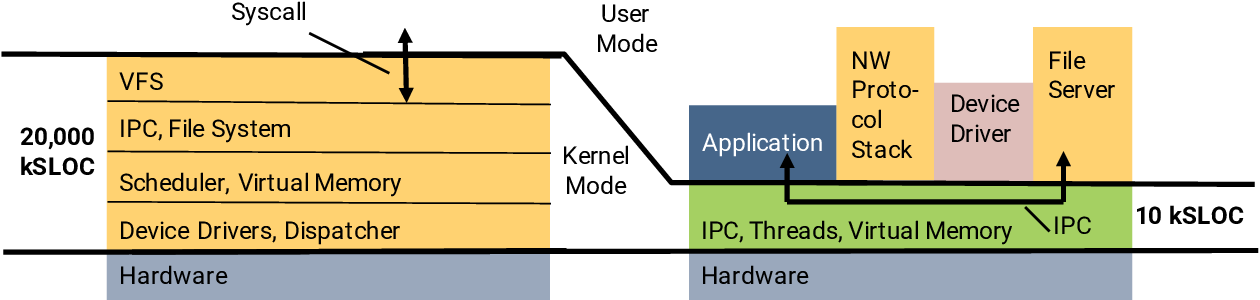
\includegraphics[width=\linewidth]{img/MonolithicVSmicrokernel.png}
  \caption{\textit{Kernel} monolitici (sinistra) VS \textit{Microkernel} (destra)}
  \label{fig:MonolithicVSmicrokernel}
\end{figure}
\newpage

\section{Scheduling della CPU}
Solitamente con il solo termine \textit{scheduling} si intende quello a breve termine della CPU, cioè la funzionalità che determina quale tra i processi (\textit{thread}) in attesa della CPU la otterranno. Chiaramente ci sono vari metodi per fare ciò, che prendono il nome di politiche di \textit{scheduling}, i quali si differenziano per modalità e prestazioni. Gli algoritmi che traducono questi metodi si chiamano algoritmi di \textit{scheduling}.

Una particolare politica di \textit{scheduling} rilevante per questo testo è \textit{Round Robin} o \textit{scheduling circolare}: consiste nel determinare un \textit{time slice} (quanto di tempo) nel quale i processi ottengono la CPU. Una volta esaurito questo tempo, il processo viene interrotto e inserito in fondo alla cosiddetta coda dei pronti. In questo modo tutti i processi ottengono la CPU per un tempo massimo stabilito; inoltre è possibile stimare il tempo di attesa prima dell'esecuzione di ciascun processo in base al numero di processi che lo precedono.

\section{Memoria virtuale}
Un altro concetto fondamentale quando si parla di sistemi operativi è la gestione della memoria. Il SO deve garantire che ogni programma abbia a disposizione la giusta quantità di memoria necessaria per l'esecuzione, ed inoltre ognuno di essi deve accedere solo alla memoria a lui riservata. Un meccanismo adottato che accomuna quanto appena detto è quello di memoria virtuale.

La memoria virtuale è un meccanismo che permette di simulare uno spazio di memoria centrale (memoria primaria) maggiore di quello fisicamente presente o disponibile, dando l'illusione all'utente di un enorme quantitativo di memoria. Questa tecnica porta con sé diversi vantaggi: uno tra questi la sicurezza dovuta all'isolamento della memoria; la possibilità di condivisione di alcune pagine di memoria tra più processi (es: le pagine contenenti le librerie possono essere usate in contemporanea da più processi senza conflitti) e infine l'ultimo, ma allo stesso tempo il principale vantaggio: avere a disposizione molta più memoria centrale di quella che in realtà è disponibile. 

Giustamente viene da chiedersi come tutto ciò sia possibile e il meccanismo alla base è quello di utilizzare una memoria ausiliaria, solitamente la memoria di massa, per allocare una certa parte di memoria che non è stata utilizzata recentemente. Nel momento in cui viene richiesta nuovamente la porzione di dati salvati nella memoria ausiliaria (oppure si libera spazio nella memoria centrale), i dati relativi vengono prelevati e copiati nuovamente in memoria centrale: questo processo prende il nome di \textit{swapping}. 

In presenza di memoria virtuale dunque non parleremo semplicemente di indirizzi di memoria, ma avremo una differenziazione tra indirizzi logici e indirizzi fisici. I programmi lavoreranno solo con indirizzi logici (quindi viene anche facilitata la programmazione) e poi a livello di CPU avverrà un processo di traduzione negli indirizzi fisici.

\section{Hypervisor}
Un tema che si distacca un po' dai concetti di base dei sistemi operativi, ma che è rilevante per la comprensione del successivo capitolo è quello di \textit{hypervisor}. Chiamato anche \textit{virtual machine monitor} (VMM), è un tipo di \textit{sotware/firmware}, che permette di creare ed eseguire macchine virtuali. Un computer sul quale un \textit{hypervisor} esegue una o più macchine virtuali viene definito \textit{host machine}, mentre le singole macchina virtuali prendono il nome di \textit{guest machine}. Su ognuna è possibile eseguire un sistema operativo (anche diverso), in modo tale che questi siano isolati tra di loro; inoltre, al contrario di un emulatore, eseguirà la maggior parte delle istruzioni direttamente sulle risorse \textit{hardware} virtualizzate rese disponibili dall'\textit{hypervisor}.